% Options for packages loaded elsewhere
\PassOptionsToPackage{unicode}{hyperref}
\PassOptionsToPackage{hyphens}{url}
%
\documentclass[
  11pt,
  ignorenonframetext,
]{beamer}
\usepackage{pgfpages}
\setbeamertemplate{caption}[numbered]
\setbeamertemplate{caption label separator}{: }
\setbeamercolor{caption name}{fg=normal text.fg}
\beamertemplatenavigationsymbolsempty
% Prevent slide breaks in the middle of a paragraph
\widowpenalties 1 10000
\raggedbottom
\setbeamertemplate{part page}{
  \centering
  \begin{beamercolorbox}[sep=16pt,center]{part title}
    \usebeamerfont{part title}\insertpart\par
  \end{beamercolorbox}
}
\setbeamertemplate{section page}{
  \centering
  \begin{beamercolorbox}[sep=12pt,center]{part title}
    \usebeamerfont{section title}\insertsection\par
  \end{beamercolorbox}
}
\setbeamertemplate{subsection page}{
  \centering
  \begin{beamercolorbox}[sep=8pt,center]{part title}
    \usebeamerfont{subsection title}\insertsubsection\par
  \end{beamercolorbox}
}
\AtBeginPart{
  \frame{\partpage}
}
\AtBeginSection{
  \ifbibliography
  \else
    \frame{\sectionpage}
  \fi
}
\AtBeginSubsection{
  \frame{\subsectionpage}
}
\usepackage{amsmath,amssymb}
\usepackage{lmodern}
\usepackage{iftex}
\ifPDFTeX
  \usepackage[T1]{fontenc}
  \usepackage[utf8]{inputenc}
  \usepackage{textcomp} % provide euro and other symbols
\else % if luatex or xetex
  \usepackage{unicode-math}
  \defaultfontfeatures{Scale=MatchLowercase}
  \defaultfontfeatures[\rmfamily]{Ligatures=TeX,Scale=1}
\fi
\usetheme[]{metropolis}
% Use upquote if available, for straight quotes in verbatim environments
\IfFileExists{upquote.sty}{\usepackage{upquote}}{}
\IfFileExists{microtype.sty}{% use microtype if available
  \usepackage[]{microtype}
  \UseMicrotypeSet[protrusion]{basicmath} % disable protrusion for tt fonts
}{}
\makeatletter
\@ifundefined{KOMAClassName}{% if non-KOMA class
  \IfFileExists{parskip.sty}{%
    \usepackage{parskip}
  }{% else
    \setlength{\parindent}{0pt}
    \setlength{\parskip}{6pt plus 2pt minus 1pt}}
}{% if KOMA class
  \KOMAoptions{parskip=half}}
\makeatother
\usepackage{xcolor}
\newif\ifbibliography
\setlength{\emergencystretch}{3em} % prevent overfull lines
\providecommand{\tightlist}{%
  \setlength{\itemsep}{0pt}\setlength{\parskip}{0pt}}
\setcounter{secnumdepth}{-\maxdimen} % remove section numbering
\ifLuaTeX
  \usepackage{selnolig}  % disable illegal ligatures
\fi
\IfFileExists{bookmark.sty}{\usepackage{bookmark}}{\usepackage{hyperref}}
\IfFileExists{xurl.sty}{\usepackage{xurl}}{} % add URL line breaks if available
\urlstyle{same} % disable monospaced font for URLs
\hypersetup{
  pdftitle={Introducción a la estadística},
  pdfauthor={Gerardo Martín},
  hidelinks,
  pdfcreator={LaTeX via pandoc}}

\title{Introducción a la estadística}
\subtitle{Encuadre}
\author{Gerardo Martín}
\date{2022-06-29}

\begin{document}
\frame{\titlepage}

\begin{frame}{Sobre mí}
\protect\hypertarget{sobre-muxed}{}
\begin{itemize}
\item
  Gerardo Martín
\item
  Veterinario
\item
  MSc Biología de Conservación

  \begin{itemize}
  \tightlist
  \item
    Modelación matemática de transmisión de enfermedades entre animales
    silvestres y domésticos
  \end{itemize}
\item
  Doctorado en Salud Pública

  \begin{itemize}
  \tightlist
  \item
    Modelación del riesgo de enfermedades emergentes de murciélagos
  \end{itemize}
\end{itemize}
\end{frame}

\begin{frame}{Sobre mí}
\protect\hypertarget{sobre-muxed-1}{}
\begin{center}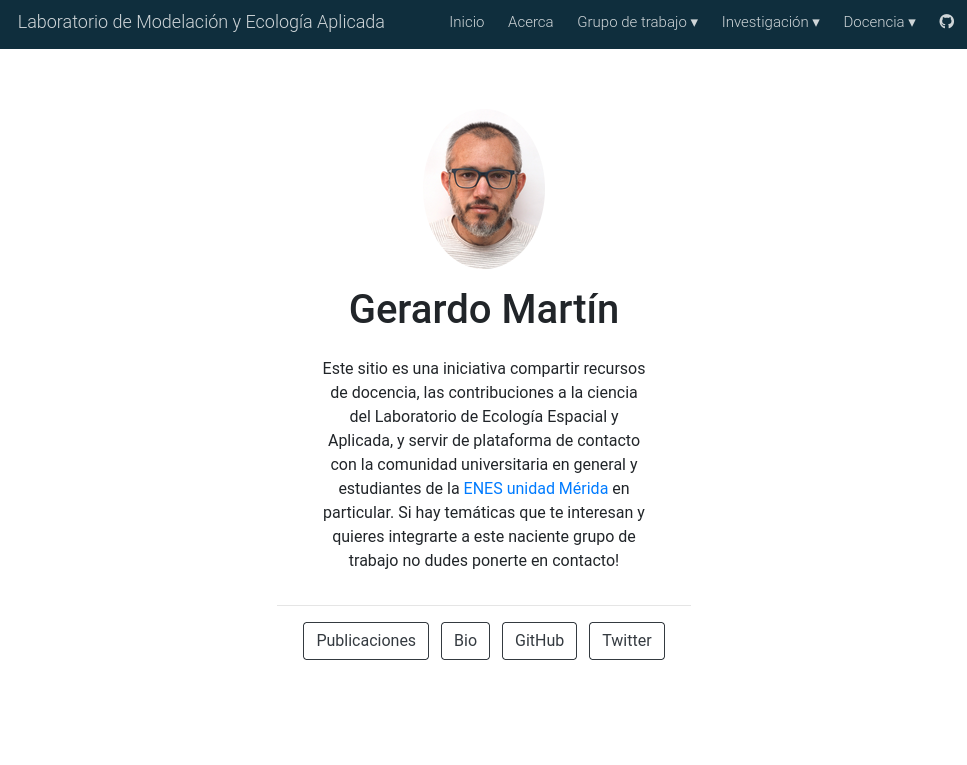
\includegraphics[width=13.43in]{Figuras Encuadre/Labo} \end{center}
\end{frame}

\begin{frame}{Contacto}
\protect\hypertarget{contacto}{}
\begin{itemize}
\tightlist
\item
  \href{mailto:gerardo.mmc@enesmerida.unam.mx}{\nolinkurl{gerardo.mmc@enesmerida.unam.mx}}
\item
  \href{https://gerardommc.github.io}{gerardommc.github.io}
\item
  \href{https://www.researchgate.net/profile/Gerardo-Martin}{ResearchGate}
\end{itemize}
\end{frame}

\begin{frame}{Sobre usted\_s}
\protect\hypertarget{sobre-usted_s}{}
\begin{itemize}
\tightlist
\item
  ¿Cómo se llaman?
\item
  ¿De dónde vienen?
\item
  ¿Qué les interesa?
\item
  ¿En qué se imaginan trabajando?
\item
  ¿Han llevado cursos de estadística?
\item
  ¿Qué esperan del curso?
\end{itemize}
\end{frame}

\begin{frame}{Sobre el curso}
\protect\hypertarget{sobre-el-curso}{}
\begin{itemize}
\item
  Introducción a la estadística:

  \begin{itemize}
  \tightlist
  \item
    Conceptos básicos y definiciones
  \item
    Plantear preguntas y planear experimentos
  \item
    Describir datos
  \item
    Aprender sobre el ambiente con datos y análisis
  \end{itemize}
\end{itemize}
\end{frame}

\begin{frame}{Contenidos del curso}
\protect\hypertarget{contenidos-del-curso}{}
\begin{enumerate}
\item
  Introducción a la estadística
\item
  Planteamiento y diseño de investigaciones
\item
  Estadística descriptiva
\item
  Inferencia estadística
\end{enumerate}
\end{frame}

\begin{frame}{Estrategia pedagógica}
\protect\hypertarget{estrategia-pedaguxf3gica}{}
\begin{itemize}
\item
  Lunes

  \begin{itemize}
  \item
    1a hora teoría
  \item
    2a hora práctica
  \end{itemize}
\item
  Viernes

  \begin{itemize}
  \item
    1a hora teoría
  \item
    2a hora retroalimentación/práctica
  \end{itemize}
\end{itemize}
\end{frame}

\begin{frame}{Lo feo \ldots{} las evaluaciones}
\protect\hypertarget{lo-feo-las-evaluaciones}{}
\begin{itemize}
\item
  Evaluación diangóstica
\item
  Evaluación formativa

  \begin{itemize}
  \tightlist
  \item
    Trabajos y retroalimentación
  \end{itemize}
\item
  Exámenes
\item
  Asistencia
\item
  Participación
\end{itemize}
\end{frame}

\begin{frame}{Las evaluaciones}
\protect\hypertarget{las-evaluaciones}{}
\begin{itemize}
\tightlist
\item
  Trabajos 50\%
\item
  Examenes 25\%
\item
  Asistencia 25\%
\item
  Participación \(\rightarrow\) extra
\end{itemize}
\end{frame}

\begin{frame}{Estrategias pedagógicas}
\protect\hypertarget{estrategias-pedaguxf3gicas}{}
\begin{itemize}
\item
  Google Classroom: izve22s
\item
  Presentaciones
\item
  Prácticas en clase

  \begin{itemize}
  \tightlist
  \item
    Calculadora
  \item
    Geogebra
  \item
    Excel
  \item
    R (introducción)
  \end{itemize}
\item
  Prácticas de tarea

  \begin{itemize}
  \tightlist
  \item
    Entregadas en GC
  \end{itemize}
\end{itemize}
\end{frame}

\hypertarget{preguntas}{%
\section{Preguntas?}\label{preguntas}}

\end{document}
